\documentclass[12pt]{article}
\usepackage{pdfpages}
\usepackage{xcolor}

\usepackage{setspace}
\onehalfspacing
\usepackage[a4paper, margin=1in]{geometry}

\title{Case Study 4 - White Collar Crime}
\author{Graham Pellegrini }
\date{\today}

\begin{document}

\maketitle
\section*{Question 1}
\textbf{Employers have often been reluctant to prosecute employees who commit crimes against them. It is easier just to fire them, thereby avoiding court hassles and bad publicity. Given that companies need to make profits, is this reluctance to bring criminal charges against employees morally permissible and responsible? (Group A Yes vs Group B No debate)}

\begin{itemize}
    \item [\textcolor{blue}{Yes}] Taking legal action consumes company time and resources. There is no financial gain in prosecuting the employee.
    
    \item [\textcolor{blue}{Yes}] Going to court might result in bad publicity for the company.

    \item [\textcolor{red}{No}] Legal action should be pursued—if not, it may create a precedent where the worst consequence is simply being fired.

    \item [\textcolor{blue}{Yes}] Just as individuals can choose not to press charges, companies should also have the right to make that decision.

    \item [\textcolor{red}{No}] If companies avoid pressing charges, the individual may continue committing crimes due to the lack of serious consequences.

    \item [\textcolor{blue}{Yes}] A proportional response is key: for minor offenses, handling it internally is appropriate; for major offenses, legal action should be taken.

    \item [\textcolor{red}{No}] The company has a moral responsibility to other employees to maintain a safe working environment.

    \item [\textcolor{blue}{Yes}] Firing an employee is still a significant punishment. It can also act as a deterrent for others who might consider similar actions.

    \item [\textcolor{blue}{Yes}] By terminating the employee, the company sets a clear internal moral standard and shows it does not support the employee's actions.

    \item [\textcolor{blue}{Yes}] The legal system is lengthy and does not guarantee a just or favorable outcome. Resolving the issue internally may be more efficient.

    \item [\textcolor{red}{No}] Publicly taking action may actually improve the company’s image. If no action is taken, it could lead to future complications, especially if the offense was severe. It may also appear suspicious, as though the company is hiding something or complicit in a larger scheme.

    \item [\textcolor{blue}{Yes}] The possibility of prosecution might create a limiting or fearful environment, discouraging creativity or open communication.

    \item [\textcolor{red}{No}] Legal consequences should only apply to employees who commit illegal actions, not affect the broader work culture.
\end{itemize}

\section*{Question 2}
\textbf{Criminal penalties for white-collar crimes have been relatively light, at least until recently. This is due, in part, to the belief that white-collar crimes are usually “victimless crimes,” since corporations rather than individuals are harmed. Are any individuals hurt in those cases, and how badly? Should those crimes be treated more lightly than crimes involving burglary, violence, or threatened violence? (Group A Yes vs Group B No debate)}

\begin{itemize}
    \item [\textcolor{blue}{Yes}] One incident of white-collar crime is not going to ruin a whole company. However a violent crime can have a much more severe impact on an individual. So the impact of each crime should be considered when determining the punishment.
    \item [\textcolor{red}{No}] White-collar crimes still create harm to a whole market and can have significant economic consequences.
    \item [\textcolor{blue}{Yes}] White-collar are crimes but there are no physical injuries. So the punishment should be less severe than crimes involving violence.
    \item [\textcolor{red}{No}] They are just as bad as these crimes are mentaly damaging as the financial loss can be devastating.
    \item [\textcolor{blue}{Yes}] Certain white-collar crimes like price fixing are actually beneficial to the economy as they stabilize prices.
    \item [\textcolor{red}{No}] White-collar crimes effect a larger pool of people.
    \item [\textcolor{red}{No}] White-collar often happening between competing companies, that often end up to the detriment of one of the companies. Which effects a large number of individuals involved. 
    \item [\textcolor{red}{No}] White-collar crimes are commited out of pure greed. While some violent crimes are commited out of necessity.
    \item [\textcolor{blue}{Yes}] Coorporations are more easily able to recover from such crimes whils individuals are not able to recover from violent crimes. Furthermore, companies have more benefits in terms of finance rather than individuals, such as the ability to write off losses and file insurance claims.
    \item [\textcolor{red}{No}] White-collar crimes settled outside of court often result in the company paying of fines which dont provide justice to the individuals affected.
\end{itemize}

\section*{Question 3}
\textbf{In the Silicon Valley case, was Catanich in an immoral conflict of interest simply by moonlighting for Gopal? (Group A: Yes vs Group B: No debate)}

\begin{itemize}
    \item [\textcolor{blue}{Yes}] Accepting money for work-related information goes against the professional code of conduct and constitutes a clear conflict of interest.
    \item [\textcolor{red}{No}] Catanich was not initially in the wrong for moonlighting, as everything was lawful until he accepted the bribe.
    \item [\textcolor{blue}{Yes}] He placed himself between two entities in the same market, potentially competitors, creating a significant conflict of interest.
    \item [\textcolor{red}{No}] He was simply using the resources and knowledge available to him to assist another company.
    \item [\textcolor{blue}{Yes}] He stole documents from his supervisor—these were not given to him, which makes the act unethical and unlawful.
    \item [\textcolor{red}{No}] Perhaps the company policies were not clearly defined, and he might not have been fully aware of the wrongdoing.
    \item [\textcolor{blue}{Yes}] Even if not explicitly written in the contract, it is considered common knowledge that one should not work for a competitor while employed.
    \item [\textcolor{red}{No}] In this line of work, it is common to moonlight or hold multiple jobs due to the nature of the industry and financial necessity.
    \item [\textcolor{blue}{Yes}] He committed theft and participated in the sale of stolen material, which escalates the situation beyond mere moonlighting.
    \item [\textcolor{blue}{Yes}] Holding two jobs is acceptable, but they should not be within the same competitive field.
    \item [\textcolor{red}{No}] It can be difficult to find work in a completely different field, as one's skillset is often specialized and doesn't easily transfer.
\end{itemize}

\section*{Question 4}
\textbf{The executives of Film Recovery Systems were convicted of murder. Critics have disagreed with this conviction on the grounds that murder involves intentional and purposeful killing. At most, say the critics, the executives committed manslaughter which is killing due to negligence or indifference (such as when drunk drivers kill). Do you think the executives of Manville should be charged with manslaughter murder, or no crime at all? (Group A Yes vs Group B No debate)}

\begin{itemize}
    \item [\textcolor{blue}{Yes}] They should be charged with man slaughter as they were aware of the damage they where cauing and as a result killed the workers indirectly.
    \item [\textcolor{blue}{Yes}] They didnt provide the neccesary equipment to the workers. Professional should always prioritize lifes.
    \item [\textcolor{red}{No}] The workers also have the responisbility on their own health and should take actions informing themselevs on what they are getting into.
    \item [\textcolor{blue}{Yes}] The fact is that they did have report and studies of what the effects of aspestos where but they decided to hide them.
    \item [\textcolor{red}{No}] The executives did not have the intent to kill, even if they put them in harms way, they didnt intend to kill them.
    \item [\textcolor{red}{No}] The executives do not bare as much responsibility as you think. Safty companies who should handle these matters have the responsibility.
    \item [\textcolor{red}{No}] From a rule utilitarian perspective, there wherent any laws in place at the time that forbided or managed aspestos.
    \item [\textcolor{blue}{Yes}] If you kill someone out of negligence it is still considered manslaughter, you are still liable.
    \item [\textcolor{blue}{Yes}] Further in the time line you see Film Recovery Systems who had a similar case in which they didn not provide proper equipment workers but ended up facing charges. Showing how the fine faced was not sufficent and they where able to get out of it by paying instead.
    \item [\textcolor{blue}{Yes}] The fact that they hide the documents proves that it is not a case of negligence.
    \item [\textcolor{red}{No}] The company did end up paying a civil payment of 2.4 billions to victims which did more good than convicting them.
    \item [\textcolor{red}{No}] Negligence from the side of the workers as they didnt follow proceecurders and didnt work mask. People in general should be more careful for their general health.
\end{itemize}
\section*{Question 5}
\textbf{One way to control white-collar crime is to use polygraph (lie detector) tests. Are companies justified in giving their employees an annual polygraph test in order to ferret out employees who are stealing from them? (Group A: Yes vs Group B: No debate)}

\begin{itemize}
    \item [\textcolor{blue}{Yes}] Polygraph tests can help identify wrongdoers before they cause potentially irreversible damage.
    \item [\textcolor{red}{No}] Presumption of innocence is a fundamental human right. Polygraph testing assumes guilt and attempts to prove it, which undermines this principle.
    \item [\textcolor{red}{No}] Polygraph tests are often inaccurate, relying on heart rate and blood pressure—factors easily influenced by stress or general anxiety.
    \item [\textcolor{red}{No}] Requiring polygraph tests may demotivate employees by creating an atmosphere of distrust.
    \item [\textcolor{red}{No}] Polygraph tests do not address root causes of misconduct, such as poor management or a toxic work environment.
    \item [\textcolor{blue}{Yes}] A single case of misconduct can affect the whole company. Since companies already monitor emails, polygraph testing can be seen as an extension of internal oversight.
    \item [\textcolor{blue}{Yes}] Polygraph testing can act as a deterrent. Knowing they may be tested could make employees think twice before engaging in illegal activities.
\end{itemize}
\footnote{The use of ChatGPT (AI Model used) was limited to the extent stated in the report.}
\pagebreak

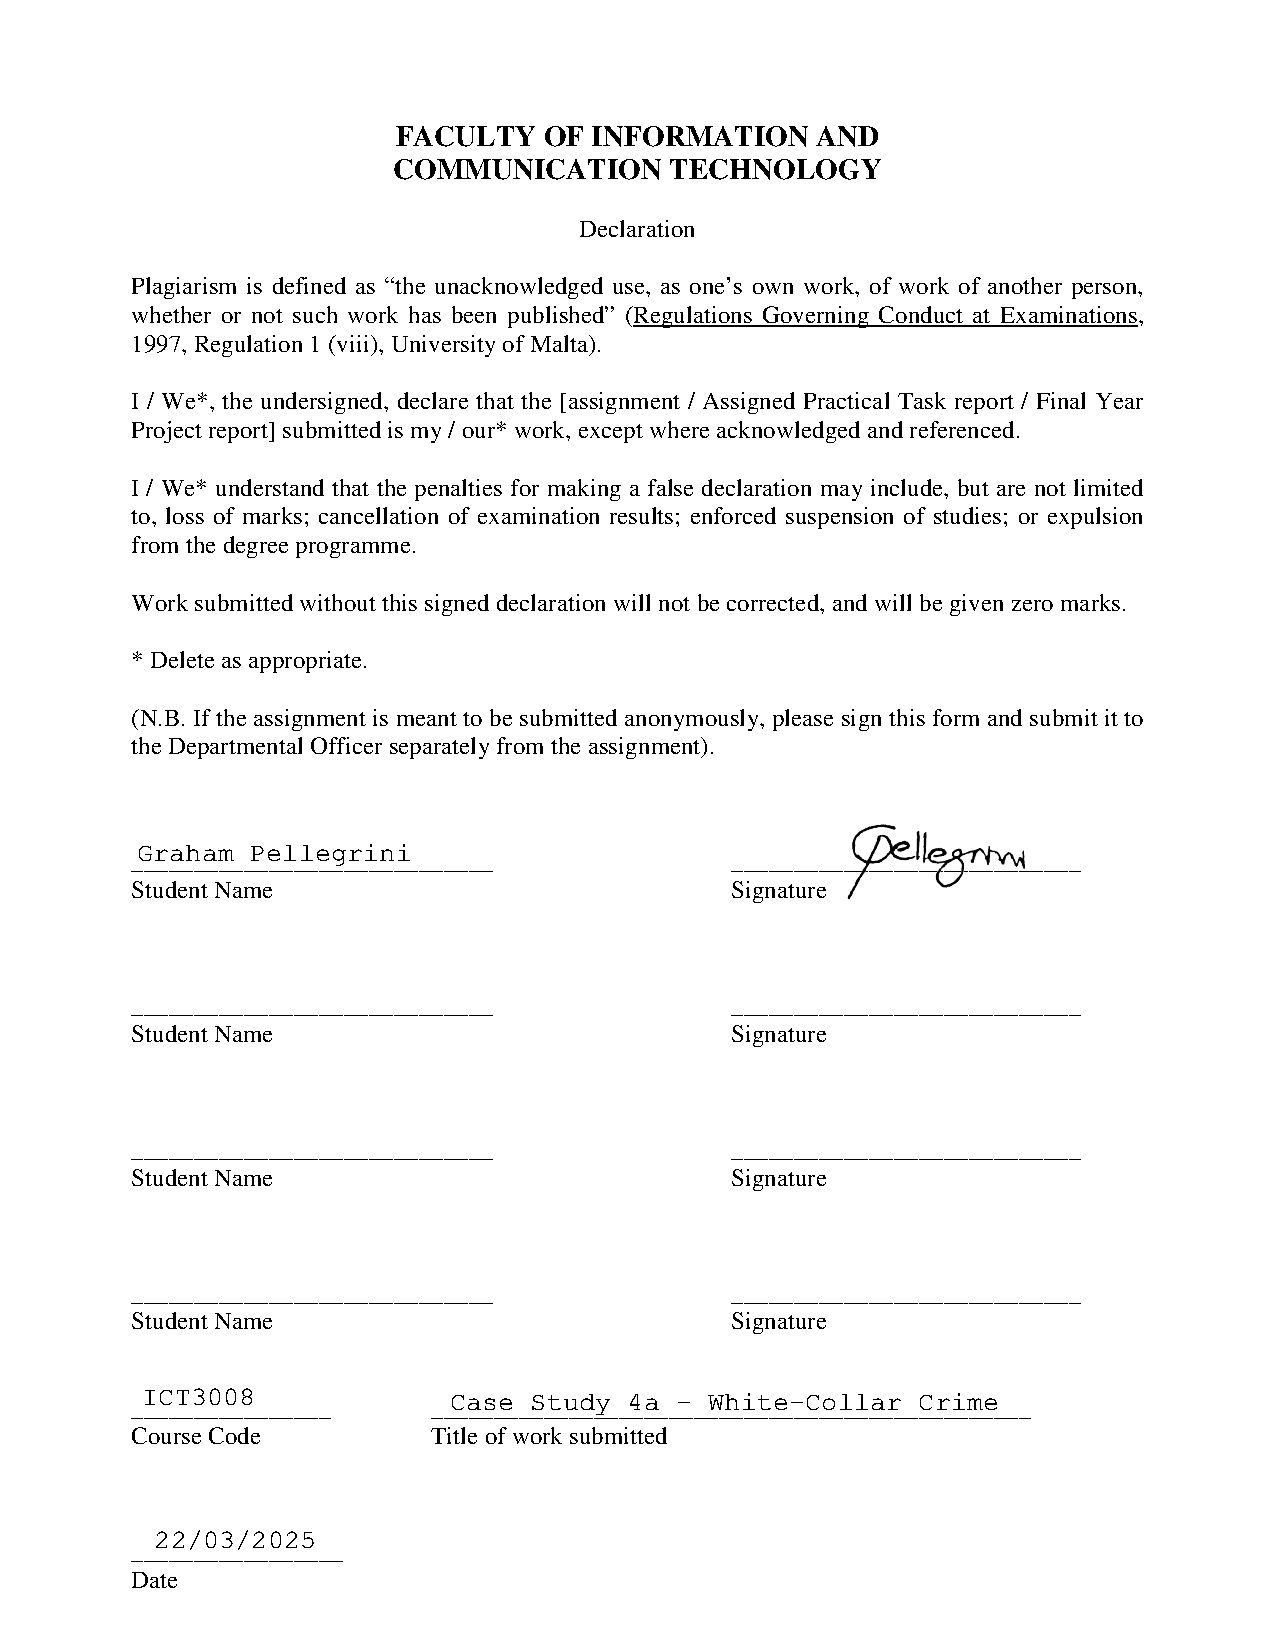
\includepdf[pages=-]{PlagiarismForm.pdf}

\end{document}



